\documentclass{beamer}

\mode<presentation>
{
  \usetheme{Frankfurt}
  \usecolortheme{orchid}
  \setbeamercovered{invisible}
  \setbeamertemplate{footline}[frame number]
}

\usepackage[english]{babel}
\usepackage[latin1]{inputenc}
\usepackage{times}
\usepackage[T1]{fontenc}
\usepackage{tikz}
\usepackage{array}

\usepackage{remreset}
\makeatletter
\@removefromreset{subsection}{section}
\makeatother
\setcounter{subsection}{1}

\title{Discrete Mathematics, Section 001, Fall 2016}
\subtitle{Lecture 1: Introduction, Definitions}
\date{September 7, 2016}

\author[Zsolt]{Zsolt Pajor-Gyulai \\ \texttt{zsolt@cims.nyu.edu}}

\pgfdeclareimage[height=1cm]{NYUlogo}{NYUlogo.jpg}

\institute[NYU] 
{
\normalsize Courant Institute of Mathematical Sciences
}
\titlegraphic{\pgfuseimage{NYUlogo}}

\begin{document}

\begin{frame}
  \titlepage
\end{frame}

\AtBeginSection[]
{
\begin{frame}
\frametitle{Outline}
\tableofcontents[currentsection]
\end{frame}}

\section{Introduction}
\subsection{Welcome to discrete mathematics}

\begin{frame}{Welcome to Discrete mathematics!}

\uncover<1->{This course is a one-semester introduction to discrete mathematics with an
emphasis on the understanding, composition and critiquing of mathematical proofs.}
\vspace{1cm}

\noindent
\uncover<2->{\begin{tabular}{l l p{2.4cm} l l}
\textbf{Instructor} & Zsolt Pajor-Gyulai\\
\textbf{Email} & zsolt@cims.nyu.edu\\
\textbf{Office} & WWH 1105A\\
\textbf{Office hours} & Mon 7:50-8:50am, 4:00-5:00pm\\
\textbf{Course Page} & via NYU Classess\\
							 ~ \\
\end{tabular}}
\vspace{0.5cm}

\uncover<3->{\textbf{Textbook:}\\
 Scheinerman, \emph{Mathematics: A Discrete Introduction. (3rd Ed)}}

\end{frame}

\begin{frame}{Welcome to Discrete mathematics!}
By the end of the course, you will (hopefully) be able to:
\begin{itemize}
\item Write clear mathematical statements using standard notation and terminology.\pause
\item Understand and execute a variety of proof techniques (contradiction, induction, etc.).\pause
\item Show fluency in the language of basic set theory and Boolean logic.\pause
\item Understand the basic theorems and their implications in a variety of (discrete) fields including:
\begin{itemize}
\item Function theory
\item Number theory
\item Graph theory
\end{itemize}
\end{itemize}
\end{frame}

\subsection{Assessment}

\begin{frame}{Written Homework (25\%)}
Distributed via \textbf{NYU Classes} site.

\begin{itemize}
\item<2-> Handwritten submission:
\begin{itemize}
\item<3-> Homeworks are \textbf{due at the beginning of the lecture at the due date}.
\item<4-> The lowest two homework score will be \textbf{dropped}. N.B. It is advised that students reserve this 'pass' for unexpected
absences.
\item<5-> In fairness to all students and graders, \textbf{no late homework} will be accepted. \textbf{No emailed homework} will be accepted.
\end{itemize}

\item<2-> PDF submission:

\begin{itemize}
\item<6->You must produce an electronic copy, \textbf{in PDF
format}. You may compose your assignment using a mathematics typesetting language like LaTeX, mathematical
software like Mathematica, or a standard word processor like Word with an equation editor.
\item<7-> No photographed handwritten work will be accepted.
\item<8-> Upload via NYU Classes.
\end{itemize}
\end{itemize}

\end{frame}

\begin{frame}{Quizzes (10\%)}
\begin{itemize}
\item Quizzes will take place in discussion sections.  \pause
\item The lowest three of these will be dropped. \pause
\item No make ups for any other reason than the ones detailed under \bf{Course Policies} below.
\end{itemize}
\end{frame}

\begin{frame}{Exams}
\begin{itemize}
\item In class Midterm 1 (20\%): October 12 \pause
\item In class Midterm 2 (20\%): November 14 \pause
\item Final (25\%): Date: December 19, 8:00-10:50am 
\end{itemize}
\end{frame}

\begin{frame}{Grades}
\vspace{-0.5cm}
\[
FS=0.25\cdot HW\%+0.1\cdot Q\%+0.2\cdot M1\%+0.2\cdot M2\%+0.25\cdot F\%
\]
\begin{center}
\begin{tabular}{c c c}
\textbf{Cutoff}&~&\textbf{Letter Grade}\\
93 & ~ &	A\\
90 &~&	A-\\
87 &~&	B+\\
83 &~&	B\\
80 &~&	B-\\
77 &~&	C+\\
70 &~&	C\\
65 &~&	D\\
\end{tabular}
\end{center}\pause
Curving:
\begin{itemize}
\item Possible, but only downwards (i.e., towards better grades).\pause
\item No information will be given out before the end of the semester.\pause
\item No letter grades are assigned to any individual midterms.
\end{itemize}
\end{frame}

\subsection{Course policies}

\begin{frame}{Qualifying reasons for accommodations}
\begin{itemize}
\item<1-> Religious holidays.
\begin{itemize}
\item<2-> Arrangements have to be made one week in advance.
\end{itemize}
\item<1-> University sponsored event.
\begin{itemize}
\item<3-> E.g. athletic tournament, play, musical performance.
\item<4-> Athletic practices or rehearsals don't qualify.
\item<5-> Arrangement have to be one week in advance.
\item<6-> Coach, conductor, or faculty advisor contact me.
\end{itemize}
\item<1-> Illness.
\begin{itemize}
\item<7-> Detailed letter from a health care provider.
\item<8-> Just stating you were there is not enough!
\end{itemize}
\end{itemize}


Note though:
\begin{itemize}
\item<9-> No homework make up, accommodation is only for submission.
\item<10-> NO ACCOMMODATION FOR MORE CONVENIENT TRAVEL!
\end{itemize}
\end{frame}

\begin{frame}{Special accomodations}
\begin{itemize}
\item Must present letter from Moses Center at the start of the course.\pause
\item Must schedule Moses Center exams a week ahead.
\end{itemize}
\end{frame}

\begin{frame}{Suggestions}
\begin{itemize}
\item \textbf{Get your hands dirty in class!}  Participate when we solve problems in class.\pause
\item \textbf{Spend time} on written assignments.  Expect each written assignment to take 4-8 hours.\pause
\item \textbf{Prepare for quizzes}, for example, by practicing on textbook problems at the end of the section.\pause
\item \textbf{Get help} early:
\begin{itemize}
\item Form study groups. \pause
\item Attend instructor and TAs' office hours. \pause
\item Use the internet, but cautiously.
\end{itemize}
\end{itemize}
\end{frame}

\begin{frame}{Stages of math education (According to Terry Tao)}
\begin{itemize}
\item<1-> \textbf{Pre-rigorous:}
\begin{itemize}
\item<2-> Informal, intuitive manner.
\item<3-> Based on examples, fuzzy notios, handwaiving.
\item<4-> Emphasis is on 'how to?' over 'why?'
\item<5-> Statement is true because teacher said so.
\item<6-> E.g. Calculus 1.
\end{itemize}
\item<1-> \textbf{Rigorous}
\begin{itemize}
\item<7-> Mathematics in a precise and formal matter.
\item<8-> Based on unambiguous statements on abstract objects.
\item<9-> Emphasis on theory. 'Why?' is the main question.
\item<10-> Statement is true because it unambiguously follows from your previous knowledge.
\item<11-> E.g. Calculus with $\epsilon-\delta$.
\end{itemize}
\item<1-> \textbf{Post-rigorous:}
\begin{itemize}
\item<12-> Comfortable with rigorous foundations of one's field.
\item<13-> Intuition is back but this time well-founded in rigorous theory.
\item<14-> Easy transition between intution and rigorous arguments.
\end{itemize}
\end{itemize}
\end{frame}

\begin{frame}{Why do rigorous math?}
\begin{block}{This class is the first step in}
\[
\textrm{Pre-rigorous}\qquad\to\qquad\textrm{Rigorous}
\]
\end{block}

\vspace{0.3cm}

This is usually rather traumatic but here is why you should do it:\vspace{-0.3cm}
\begin{itemize}
\item Pre-rigorous approach becomes inadequate as complexity of the subject increases.
\item We need to be able to tell if a statement is true, even if it is not obvious by immediate intuition. 
\item This can be done through a chain of obviously true implications from an obviously true statement (\alert{Proof}).
\end{itemize}
\begin{figure}
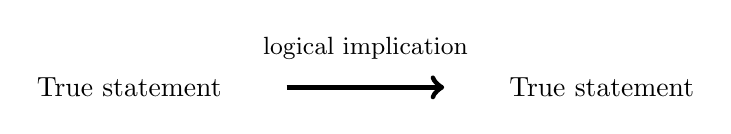
\begin{tikzpicture}
\node at (0,2) {True statement};
\draw[line width=2pt, ->] (2,2) -- (4,2);
\node at (6,2) {True statement};
\node at (3,2.5) {\small{logical implication}};
\end{tikzpicture}
\end{figure}
\end{frame}


\section{Definitions}

\begin{frame}{What is a mathematical definition?}
\begin{itemize}
\item Mathematical objects are purely conceptual and come to existence by precise definitions.\pause
\item This is done in an unambiguous way, in terms of previously well defined mathematical objects using English.
\end{itemize}\pause

\vspace{0.5cm}
 For example:
\begin{definition}
An integer is called \textbf{even} provided it is divisible by two.
\end{definition}\pause

\vspace{0.5cm}
\center{What are integer, divisible, two?}
\end{frame}

\begin{frame}{Fundamental objects (for this class)}
Some objects and their properties have to be considered given. 
\begin{itemize}
\item \underline{Numbers:}
\begin{itemize}
\item \textbf{Natural numbers:} $\mathbb{N}=\{0,1,2,3,\dots\}$
\item \textbf{Integer numbers:} $\mathbb{Z}=\{\dots, -3,-2,-1,0,1,2,3,\dots\}$
\item \textbf{Rational numbers:} $\mathbb{Q}$
\item \textbf{Real numbers:} $\mathbb{R}$
\end{itemize}
\item \underline{Operations:} $+,\cdot$.
\item \underline{Order relations:} $<,\leq,>,\geq,=$.
\end{itemize}

\vspace{1cm}
If you want to dig deeper: \alert{Mathematical logic}
\end{frame}

\begin{frame}
\begin{definition}
An integer is called \textbf{even} provided it is divisible by two.
\end{definition}\pause

\begin{itemize}
\item No need to define integer or two.
\item However, what does divisible mean?
\end{itemize}
e.g. Is $3$ divisible by 2?
\[
\textrm{'$3$ ~~divided by~~ $2$~~ is~~ $\frac{3}{2}$.'}
\]
But this is not what we want!

\begin{definition}
Let $a$ and $b$ integers. We say that $a$ is \textbf{divisible} by $b$ provided there is an integer $c$ such that $bc=a$. 
\end{definition}
\end{frame}

\begin{frame}[t]

\begin{definition}
Let $a$ and $b$ integers. We say that $a$ is \textbf{divisible} by $b$ provided there is an integer $c$ such that $bc=a$. 
\end{definition}

For example:
\begin{itemize}
\only<2>{\item Is $12$ divisible by $4$?}
\item<3->$12$ is divisible by $4$ because there is an integer $3$ such that $4\cdot 3=12$.
\only<4>{\item Is $12$ divisible by $5$?}
\item<5-> $12$ is not divisible by $5$ because there is no integer $x$ for which $5x=12$.
\end{itemize}
\uncover<6>{\begin{block}{Terminology and notation}
If $a$ is divisible by $b$, we write $b|a$ and also say
\begin{itemize}
\item $b$ divides $a$,
\item $b$ is a factor of $a$,
\item $b$ is a divisor of $a$.
\end{itemize}
\end{block}}
\end{frame}

\begin{frame}
\begin{definition}
An integer is called \textbf{even} provided it is divisible by two.
\end{definition}

What about odd numbers?

\begin{block}{Alternative 1}
An integer $a$ is called \textbf{odd} provided it is not even.
\end{block}

\begin{block}{Alternative 2 (We go with this one)}
An integer $a$ is called \textbf{odd} provided there is an integer $x$ such that $a=2x+1$.
\end{block}

\center{\alert{That these two are equivalent is a statement that requires verification!}}
\end{frame}

\begin{frame}[t]
\vspace{1.5cm}
\begin{definition}
An integer is called \textbf{even} provided it is divisible by two.
\end{definition}
\begin{definition}
An integer $a$ is called \textbf{odd} provided there is an integer $x$ such that $a=2x+1$.
\end{definition}
For example:
\begin{itemize}
\only<1>{\item Is $12$ even?}
\item<2-> $12$ is even because $2\cdot 6 = 12$.
\only<3>{\item Is $13$ odd?}
\item<4-> $13$ is odd because $2\cdot 6 + 1 = 13$.
\end{itemize}
\end{frame}

\begin{frame}[t]{Prime numbers, composite numbers}
\vspace{0.5cm}
\begin{definition}
An integer $p$ is called \textbf{prime} provided $p>1$ and the only positive divisors of $p$ are $1$ and $p$.
\end{definition}

For example:
\begin{itemize}
\only<2>{\item Is $11$ a prime?}
\item<3-> $11$ is a prime because $11>1$ and the only positive divisors are $1$ and $11$.
\only<4>{\item Is $12$ a prime?}
\item <5-> $12$ is not a prime because $3|12$ and $3\neq 1$ or $12$.
\only<6>{\item Is $1$ a prime number?}
\item <7-> $1$ is not a prime because $1\ngtr1$.
\end{itemize}
\end{frame}

\begin{frame}[t]{Prime numbers, composite numbers}
\vspace{0.5cm}
\begin{definition}
A positive integer $a$ is called \textbf{composite} provided there is an integer $b$ such that $1<b<a$ and $b|a$.
\end{definition}
For example:
\begin{itemize}
\only<2>{\item Is $12$ a composite number?}
\item<3-> $12$ is a composite number because e.g. $1<3<12$ and $3|12$.
\only<4>{\item Is $360$ a composite number?}
\item<5-> $360$ is a composite number as e.g. $1<180<360$ and $180|360$.
\only <6>{\item Is $1$ a composite number?}
\item<7-> $1$ is not a composite number as there is no number $b$ such that $1<b<1$.
\end{itemize}
\end{frame}

\begin{frame}{Prime numbers, composite numbers}
\begin{definition}
An integer $p$ is called \textbf{prime} provided $p>1$ and the only positive divisors of $p$ are $1$ and $p$.
\end{definition}

\begin{definition}
A positive integer $a$ is called \textbf{composite} provided there is an integer $b$ such that $1<b<a$ and $b|a$.
\end{definition}
Comparison:
\begin{itemize}
\item A prime $p$ is not composite as there is no integer $b$ with $1<b<p$ with $b|p$.\pause
\item A composite $a$ is not a prime as there is an integer $b\neq 1,a$ such that $b|a$.\pause
\item However, $1$ is neither a prime, nor a composite.
\end{itemize}
\end{frame}







\end{document}